\section{Structure générale}
Vigilate est une solution composé de 3 programmes différents :\\
\begin{itemize}
\item Un site web\\
\item Un scanner\\
\item Un backend\\
\end{itemize}
Vigilate pourra optionnellement être distribué sur une vm.\\
\section{Le site web}
Le site web servira à la personnalisation des alertes. On pourra choisir quels programmes suivre. On pourra aussi choisir un niveau de criticité minimum par programme pour être prévenue. Le site permettra aussi de choisir le ou les moyens par lesquels on veut être prévenue lors de la découverte d’une vulnérabilité (mail, sms ou notifications sur le site). Le site web enverra ces données au backend via l’api pour qu’il mette à jour la base de donnée.\\

\section{Le scanner de programme}
Le scanner de programme est là par soucis de simplicité d’utilisation, ce sera un programme en python (donc portable) qui récupérera la liste des programmes installés et les enverra au backend via l’api pour mettre à jours la base de données. Le scann pourra être lancer manuellement ou planifier pour s’exécuter régulièrement (par exemple un fois par semaine).\\

\section{Le Backend}
Le backend, ce sera le coeur de vigilate. C’est un programme qui récupérera les cve dès leurs sortie via le flux rss du site cve.mitre.org. Une fois récupéré il les stockera dans la base de données et regardera si un des clients utilise ce programme, si c’est le cas il vérifiera ensuite si la version est vulnérable. Puis il ira voir si le niveau de criticité est égale ou supérieur à celui préciser par le client via le site web, si c’est le cas il préviendra le client par tout les moyens que celui-ci aura choisit.\\
Le backend recevra aussi  les informations du scanneur et les stockera dans une base de données.\\
Le backend hébergera aussi l’api de vigilate, cette api permettra au backend de communiquer avec le scanneur et le site web, elle récupérera leur requêtes et fera les modifications nécessaires dans la base de données. L’api permettra de modifier la liste de programmes installés et leurs versions ainsi que de changer les préférences (niveau de criticité et moyen de contact).\\

\section{La vm}
Pour finir Vigilate aura optionnellement une vm. Ce sera machine virtuelle prête à fonctionner qui contiendra le site web et le backend de vigilate. Un système de mise à jours permettra à la vm d’avoir les composants de vigilate toujours à jours sans avoir à la réinstaller.\\

\section{Cas d’utilisation}
\begin{figure}[]
  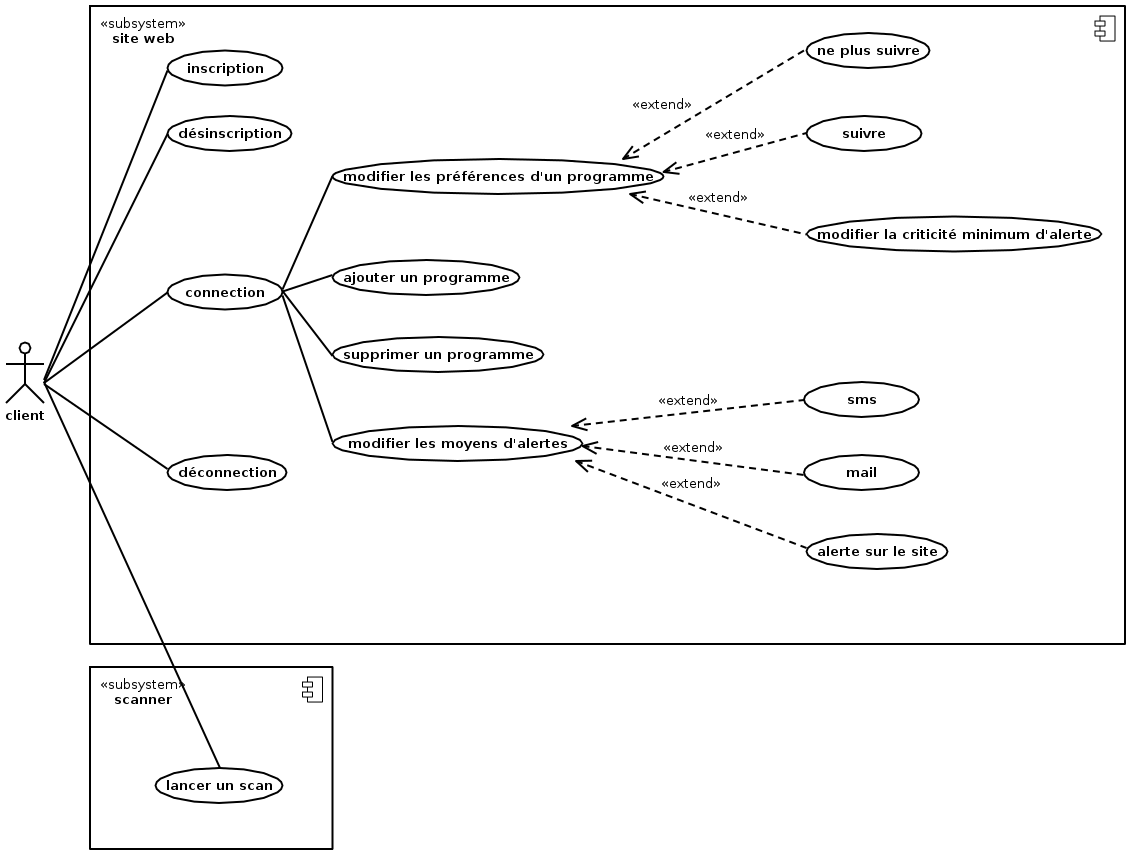
\includegraphics[width=18cm]{uml1.png}
\end{figure}
\begin{figure}[]
  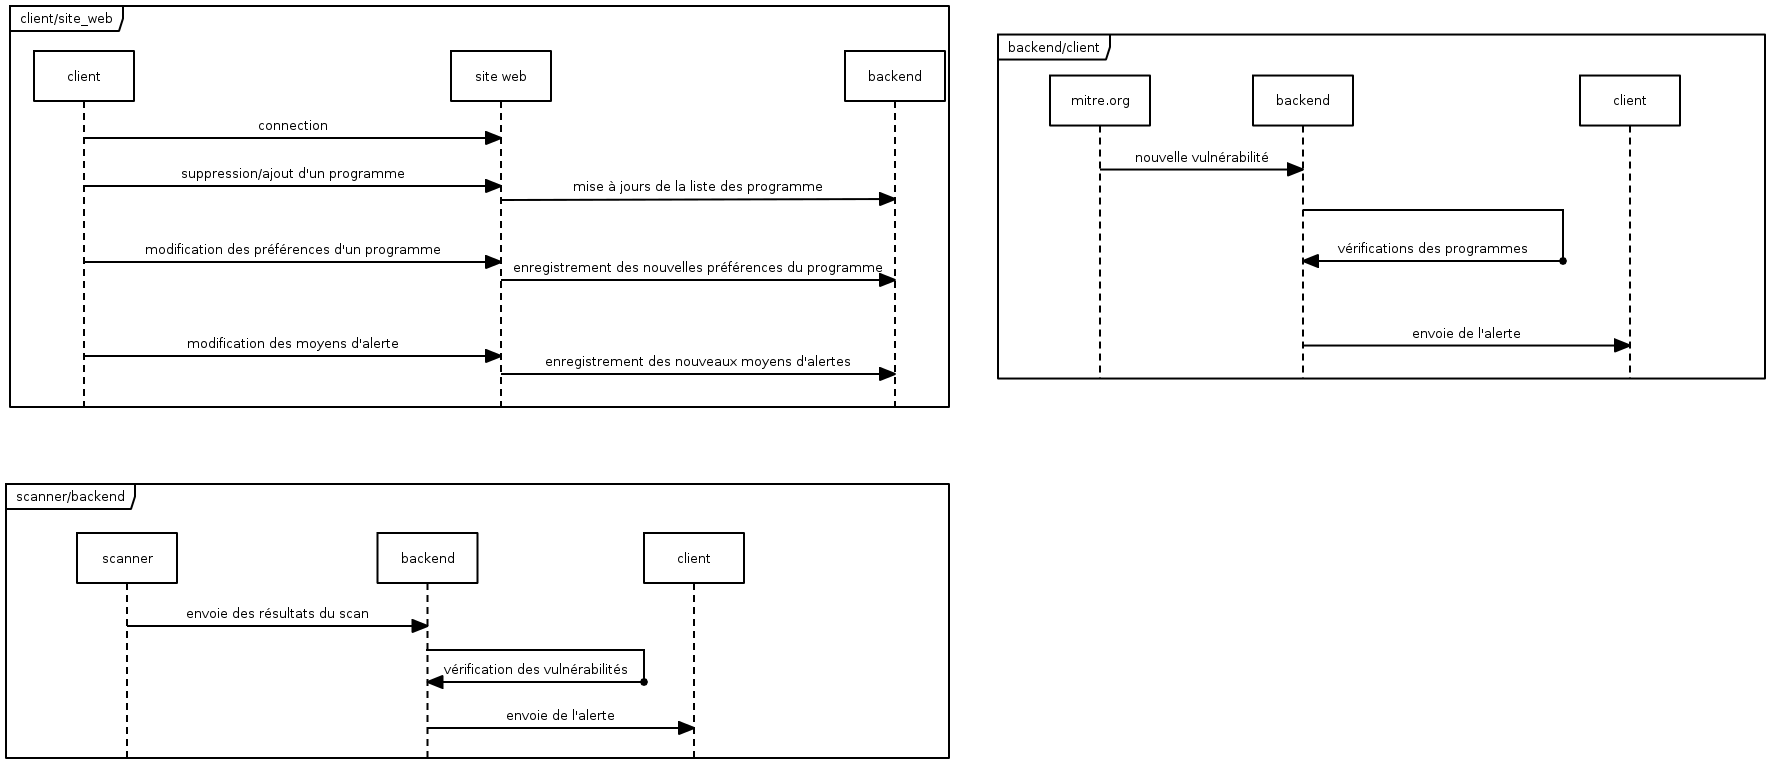
\includegraphics[width=18cm]{uml2.png}
\end{figure}
